% Figure 2 of the ISMRM 2027 abstract, kept as close as possible to the original
% diagrams: (A) presentation/envloop_diagram.tex, (B) presentation/controller_diagram.tex.
% Only code references, the action and observation labels, and "held-out" were
% changed. Defining \logicfix before loading this file draws the lookahead as it
% runs in python/train_e2_mf.py (an extra early-promotion check; plateau promotes
% on its own). Build both variants with scripts/fig2_loops_minimal.sh.
\documentclass[border=6pt]{standalone}
\usepackage{tikz}
\usepackage{amsmath}
\usetikzlibrary{positioning,arrows.meta,fit,calc,backgrounds,shapes.geometric}

% New brand ImperialBlue (from ic_eee_thesis.cls)
\definecolor{ImperialBlue}{RGB}{0,0,205}
\definecolor{V2accent}{RGB}{200,80,0}     % orange accent for the lookahead check

\newif\iflogicfix
\ifdefined\logicfix\logicfixtrue\fi

\begin{document}
\begin{tabular}{@{}c@{}}
% =============================== (A) env loop ===============================
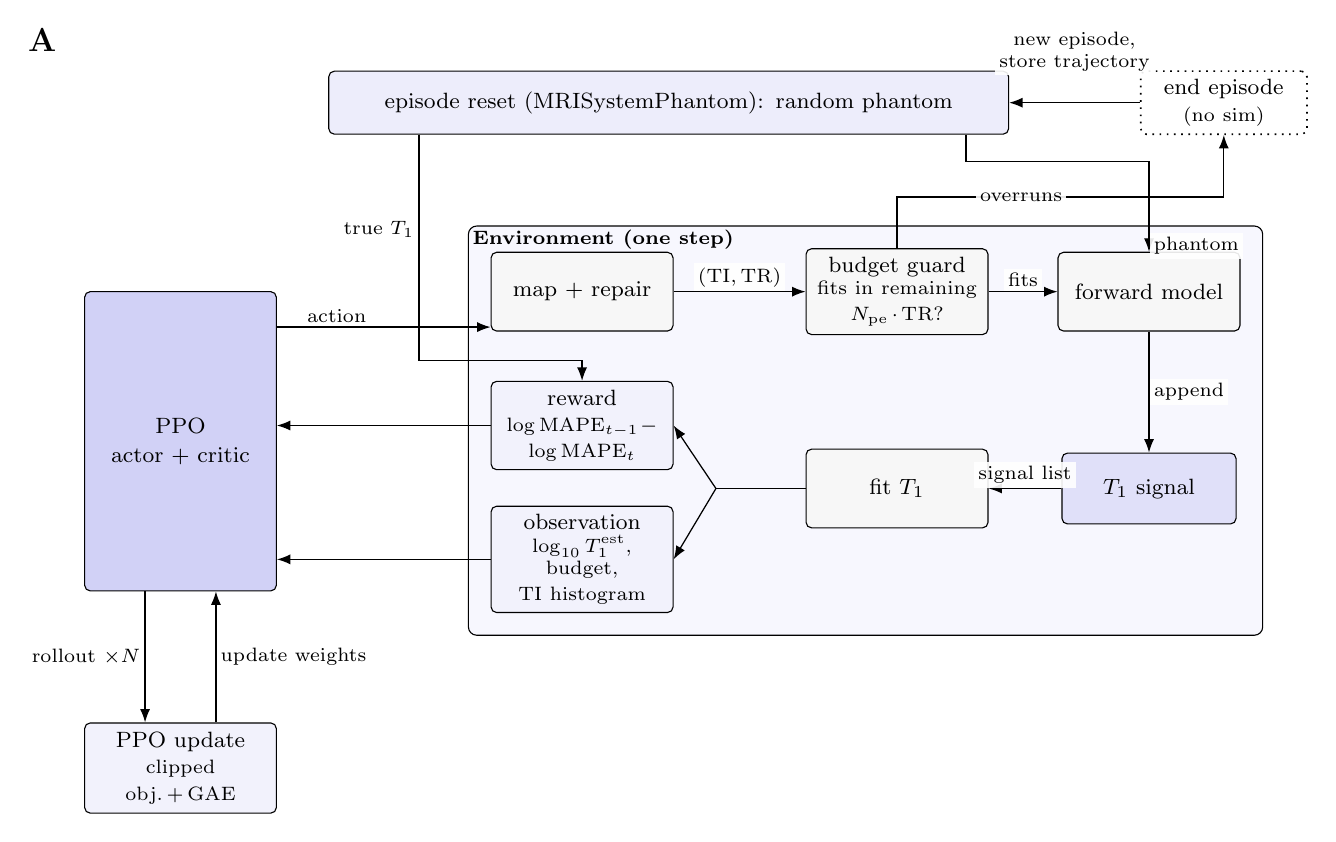
\begin{tikzpicture}[
  font=\footnotesize,
  proc/.style={draw, rounded corners=2pt, align=center, inner xsep=3pt,
    inner ysep=3pt, minimum height=10mm, text width=21mm, fill=black!3},
  state/.style={draw, rounded corners=2pt, align=center, inner xsep=3pt,
    inner ysep=3pt, minimum height=9mm, text width=20mm, fill=ImperialBlue!12},
  io/.style={draw, rounded corners=2pt, align=center, inner xsep=3pt,
    inner ysep=3pt, minimum height=9mm, text width=21mm, fill=ImperialBlue!5},
  endb/.style={draw, dotted, line width=0.6pt, rounded corners=2pt, align=center,
    inner xsep=3pt, inner ysep=3pt, minimum height=8mm, text width=19mm},
  agent/.style={draw, rounded corners=2pt, align=center, fill=ImperialBlue!18,
    text width=22mm, minimum height=38mm},
  reset/.style={draw, rounded corners=2pt, align=center, fill=ImperialBlue!7,
    text width=84mm, minimum height=8mm},
  upd/.style={draw, rounded corners=2pt, align=center, fill=ImperialBlue!5,
    text width=22mm, minimum height=9mm},
  arr/.style={-{Latex[length=1.7mm]}, line width=0.45pt},
  lbl/.style={font=\scriptsize, inner sep=1.5pt, fill=white, fill opacity=0.9,
    text opacity=1},
]
\node[agent] (ppo) at (0,1.0) {PPO\\[1pt] actor $+$ critic};
\node[upd] (update) at (0,-3.15) {PPO update\\ \scriptsize clipped obj.\,$+$\,GAE};

\node[proc] (map)   at (5.1,2.9)  {map $+$ repair};
\node[proc] (guard) at (9.1,2.9)  {budget guard\\ \scriptsize fits in remaining\\ $N_\mathrm{pe}\!\cdot\!\mathrm{TR}$?};
\node[proc] (fwd)   at (12.3,2.9) {forward model};

\node[io] (rew) at (5.1,1.2)  {reward\\ \scriptsize $\log\mathrm{MAPE}_{t-1}\!-\!\log\mathrm{MAPE}_t$};
\node[io] (obs) at (5.1,-0.5) {observation\\ \scriptsize $\log_{10}T_1^{\mathrm{est}}$, budget,\\ TI histogram};

\node[state] (sig) at (12.3,0.4) {$T_1$ signal};
\node[proc]  (fit) at (9.1,0.4)  {fit $T_1$};

\node[reset] (reset) at (6.2,5.3)
  {episode reset (MRISystemPhantom): random phantom};
\node[endb] (end) at (13.25,5.3) {end episode\\ \scriptsize (no sim)};

\begin{scope}[on background layer]
\node[draw, rounded corners=3pt, fill=ImperialBlue!3, inner sep=8pt,
      fit=(map)(guard)(fwd)(sig)(fit)(rew)(obs)] (envbox) {};
\node[lbl, anchor=north west, fill=none] at (envbox.north west) {\textbf{Environment (one step)}};
\end{scope}

\coordinate (actionout) at ($(ppo.east)+(0,1.45)$);
\draw[arr] (actionout) -- (map.west|-actionout)
  node[lbl, pos=0.28, above] {action};
\draw[arr] (map) -- (guard) node[lbl, midway, above] {\scriptsize$(\mathrm{TI},\mathrm{TR})$};
\draw[arr] (guard) -- (fwd) node[lbl, midway, above] {fits};

\draw[arr] (guard.north) -- ++(0,0.65) -| (end.south)
  node[lbl, pos=0.12, right] {overruns};
\draw[arr] (end.west) -- (reset.east)
  node[lbl, midway, align=center, yshift=6.5mm] {new episode,\\ store trajectory};

\coordinate (phantomout) at ($(reset.south east)+(-0.55,0)$);
\draw[arr] (phantomout) -- ++(0,-0.34) -| (fwd.north)
  node[lbl, pos=0.88, right, yshift=-2mm] {phantom};
\coordinate (t1bus) at ($(envbox.west)+(-0.62,0)$);
\coordinate (t1drop) at ($(rew.north)+(0,0.26)$);
\draw[arr] (reset.south-|t1bus) --
  node[lbl, pos=0.42, left] {true $T_1$}
  (t1bus|-t1drop) -- (t1drop) -- (rew.north);

\draw[arr] (fwd.south) -- (sig.north) node[lbl, midway, right] {append};
\draw[arr] (sig) -- (fit) node[lbl, midway, above] {signal list};
\coordinate (fork) at (6.8,0.4);
\draw (fit.west) -- (fork);
\draw[arr] (fork) -- (rew.east);
\draw[arr] (fork) -- (obs.east);

\draw[arr] (rew.west) -- (ppo.east|-rew);
\draw[arr] (obs.west) -- (ppo.east|-obs);

\draw[arr] ($(ppo.south)+(-0.45,0)$) -- ($(update.north)+(-0.45,0)$)
  node[lbl, midway, left] {rollout $\times N$};
\draw[arr] ($(update.north)+(0.45,0)$) -- ($(ppo.south)+(0.45,0)$)
  node[lbl, midway, right] {update weights};

\node[anchor=north west, font=\large\bfseries, inner sep=0pt]
  at (current bounding box.north west) {A};
\end{tikzpicture}
\\[3mm]
% ============================ (B) MF controller =============================
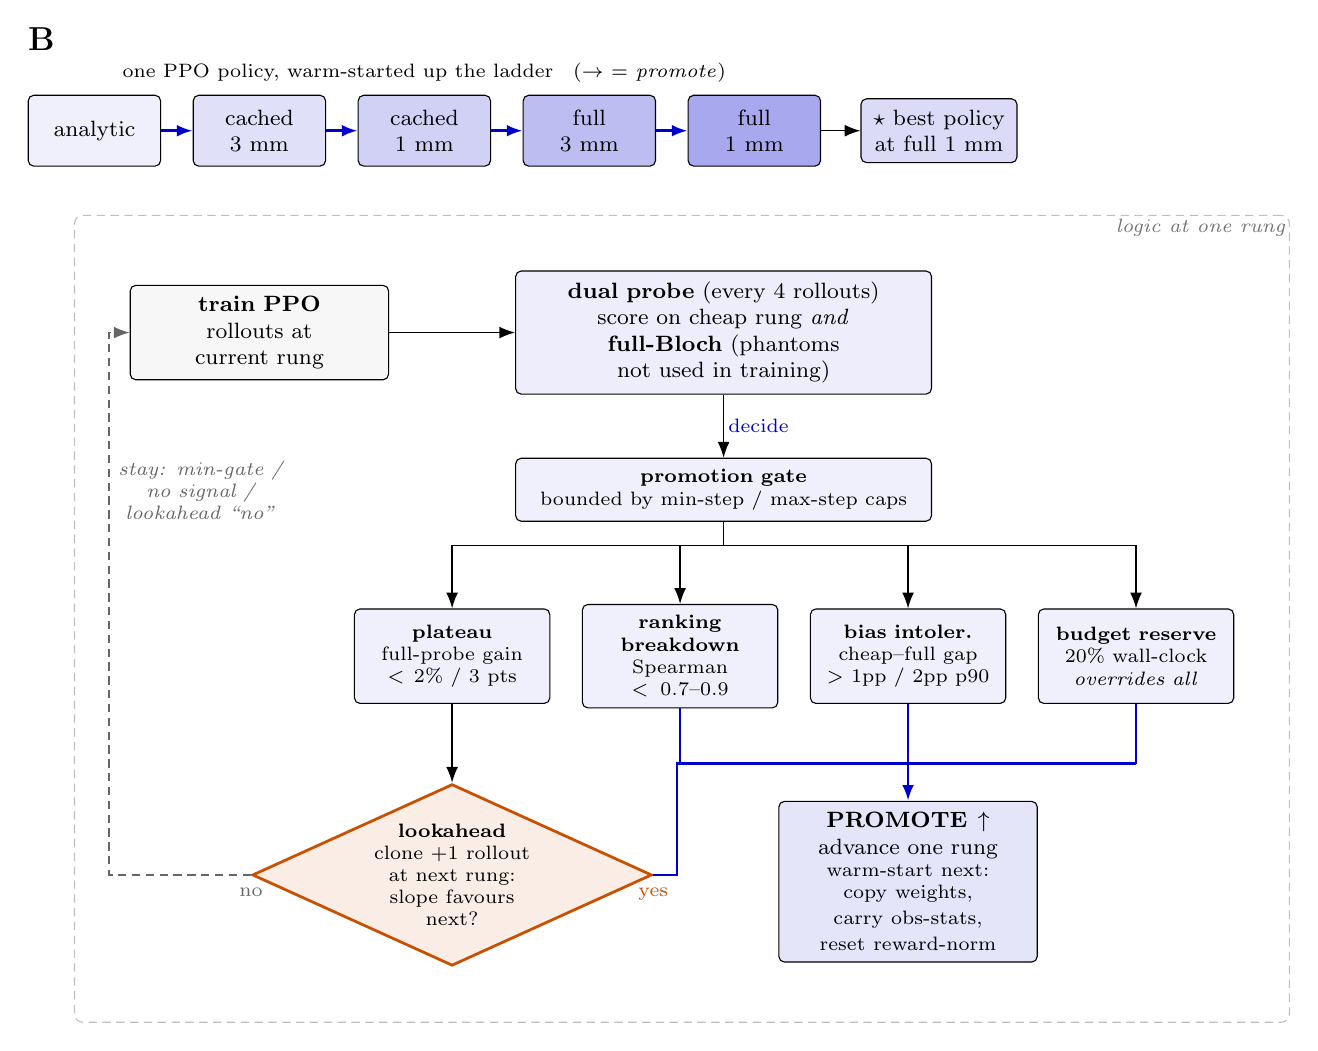
\begin{tikzpicture}[
  font=\footnotesize,
  >={Latex[length=2mm]},
  box/.style={draw, rounded corners=2pt, align=center, inner sep=4pt, minimum height=8mm},
  rung/.style={box, text width=14mm, minimum height=9mm, font=\footnotesize},
  proc/.style={box, fill=black!3, text width=30mm},
  probe/.style={box, fill=ImperialBlue!7, text width=50mm},
  sig/.style={box, fill=ImperialBlue!6, text width=22mm, font=\scriptsize, minimum height=12mm},
  v2/.style={draw=V2accent, line width=1pt, fill=V2accent!10, diamond, aspect=2.2,
             align=center, inner sep=1pt, font=\scriptsize, text width=20mm},
  gate/.style={box, fill=ImperialBlue!6, text width=50mm, font=\scriptsize},
  arr/.style={->, line width=0.5pt},
  promote/.style={->, line width=1pt, ImperialBlue},      % directed (with head)
  promoteline/.style={line width=1pt, ImperialBlue},      % joining segment (no head)
  stay/.style={->, line width=0.6pt, densely dashed, black!60},
  lbl/.style={font=\scriptsize, inner sep=1.5pt},
  plbl/.style={font=\scriptsize, inner sep=1.5pt, ImperialBlue},
]

% ============ LADDER SPINE (top) ============
\node[rung, fill=ImperialBlue!6]  (r1) {analytic};
\node[rung, right=4mm of r1, fill=ImperialBlue!12] (r2) {cached\\ 3 mm};
\node[rung, right=4mm of r2, fill=ImperialBlue!18] (r3) {cached\\ 1 mm};
\node[rung, right=4mm of r3, fill=ImperialBlue!26] (r4) {full\\ 3 mm};
\node[rung, right=4mm of r4, fill=ImperialBlue!34] (r5) {full\\ 1 mm};
\node[box, right=5mm of r5, fill=ImperialBlue!14, text width=17mm, font=\footnotesize]
      (star) {$\star$ best policy\\ at full 1 mm};
\draw[promote] (r1)--(r2);
\draw[promote] (r2)--(r3);
\draw[promote] (r3)--(r4);
\draw[promote] (r4)--(r5);
\draw[arr] (r5)--(star);
\node[lbl, above=1mm of r3.north] {one PPO policy, warm-started up the ladder \;\;($\rightarrow$ = \textit{promote})};

% ============ INNER LOOP (logic at the current rung) ============
\node[proc, below=15mm of r2.south] (train) {\textbf{train PPO}\\ rollouts at current rung};
\node[probe, right=16mm of train] (probe)
   {\textbf{dual probe} (every 4 rollouts)\\ score on cheap rung \emph{and}\\ \textbf{full-Bloch} (phantoms not used in training)};
\draw[arr] (train) -- (probe);

% Gate band
\node[gate, below=8mm of probe] (gate)
   {\textbf{promotion gate}\\ \scriptsize bounded by min-step / max-step caps};
\draw[arr] (probe) -- (gate)
      node[plbl, midway, right] {decide};

% the four signals (any one fires => promote)
\node[sig, below left=11mm and 22mm of gate.south] (plateau) {\textbf{plateau}\\ full-probe gain\\ $<2\%$ / 3 pts};
\node[sig, right=4mm of plateau] (rank)    {\textbf{ranking}\\ \textbf{breakdown}\\ Spearman $<0.7$--$0.9$};
\node[sig, right=4mm of rank]    (bias)    {\textbf{bias intoler.}\\ cheap--full gap\\ $>1$pp / $2$pp p90};
\node[sig, right=4mm of bias]    (budget)  {\textbf{budget reserve}\\ 20\% wall-clock\\ \emph{overrides all}};
\draw[arr] (gate.south) -- ++(0,-3mm) -| (plateau.north);
\draw[arr] (gate.south) -- ++(0,-3mm) -| (rank.north);
\draw[arr] (gate.south) -- ++(0,-3mm) -| (bias.north);
\draw[arr] (gate.south) -- ++(0,-3mm) -| (budget.north);

% lookahead decision on the plateau branch
\node[v2, below=10mm of plateau, xshift=0mm] (v2)
     {\textbf{lookahead}\\ clone $+1$ rollout\\ at next rung:\\ slope favours next?};
\iflogicfix
\draw[arr] (plateau) -- (v2) node[plbl, V2accent, midway, left] {early-promotion check};
\else
\draw[arr] (plateau) -- (v2);
\fi

% ---- collector bus: one arrowhead total (into PROMOTE) ----
\coordinate (busy) at ($(rank.south)+(0,-7mm)$);
% direct signals drop onto the bus (no heads)
\draw[promoteline] (rank.south)   -- (rank.south   |- busy);
\draw[promoteline] (bias.south)   -- (bias.south   |- busy);
\draw[promoteline] (budget.south) -- (budget.south |- busy);
\iflogicfix
% plateau promotes on its own, like the other signals
\draw[promoteline] ([xshift=5mm]plateau.south) -- ([xshift=5mm]plateau.south |- busy)
                   -- (rank.south |- busy);
\fi
% lookahead "yes" joins from the right (no head)
\draw[promoteline] (v2.east) -- ++(3mm,0) |- (bias.south |- busy);
\node[plbl, V2accent, below=3pt of v2.east] {yes};
% horizontal bus
\draw[promoteline] (rank.south |- busy) -- (budget.south |- busy);
% single directed exit into PROMOTE
\coordinate (sigmid) at ($(rank.south)!0.5!(budget.south)$);
\node[box, fill=ImperialBlue!10, text width=30mm, font=\footnotesize]
     (promoteout) at ($(sigmid |- busy) + (0,-15mm)$)
     {\textbf{PROMOTE}\;\,$\uparrow$ advance one rung\\ \scriptsize warm-start next: copy weights,\\ carry obs-stats, reset reward-norm};
\draw[promote] (sigmid |- busy) -- (promoteout.north);

% lookahead "no" exits LEFT -> short left-gutter stay loop back to train
\draw[stay] (v2.west) -- ++(-18mm,0) |- (train.west);
\node[lbl, black!60, below=3pt of v2.west] {no};
\iflogicfix
\node[lbl, black!60, anchor=center, align=center, text width=22mm]
      at ($(train.west)+(+9mm,-20mm)$)
      {\itshape stay: min-gate,\\ or no signal and\\ lookahead ``no''};
\else
\node[lbl, black!60, anchor=center, align=center, text width=22mm]
      at ($(train.west)+(+9mm,-20mm)$)
      {\itshape stay: min-gate /\\ no signal / lookahead ``no''};
\fi

% dashed enclosure to mark "the logic at one rung"
\begin{scope}[on background layer]
\node[draw=black!25, densely dashed, rounded corners=3pt, inner sep=7mm,
      fit=(train)(probe)(gate)(plateau)(budget)(v2)(promoteout)] (loopbox) {};
\end{scope}
\node[lbl, anchor=north east, black!55] at (loopbox.north east) {\itshape logic at one rung};

\node[anchor=north west, font=\large\bfseries, inner sep=0pt]
  at ([yshift=4mm]current bounding box.north west) {B};
\end{tikzpicture}
\end{tabular}
\end{document}
